% !TeX root = ../main.tex

\chapter{工具实现与评估}
\label{sec:实验与评估}

本章将分别介绍第\ref{sec:区间算数}章和第\ref{sec:值流图}章所述方法的模块实现与评估方法。

\section{基于区间代数的整数缺陷检测方法的实现与评估}
\label{sec:区间算数评估与结果}

\subsection{模块实现} 
\label{sec:区间算数模块实现}

我们选择在静态分析框架Tsmart-V3上实现第\ref{sec:区间算数}章节所述抽象域与算法。Tsmart-V3基于开源的静态分析框架CPAChecker,在此基础上进行大量的优化与修改,同时提供了相比CPAChecker更加丰富的行为接口与更为丰富的文档。工具使用的编程语言为Java,目标检测语言是C语言。

整体的工具的架构设计如图\ref{fig:整型分析架构图}所示。

\begin{figure}[H]
	\centering
	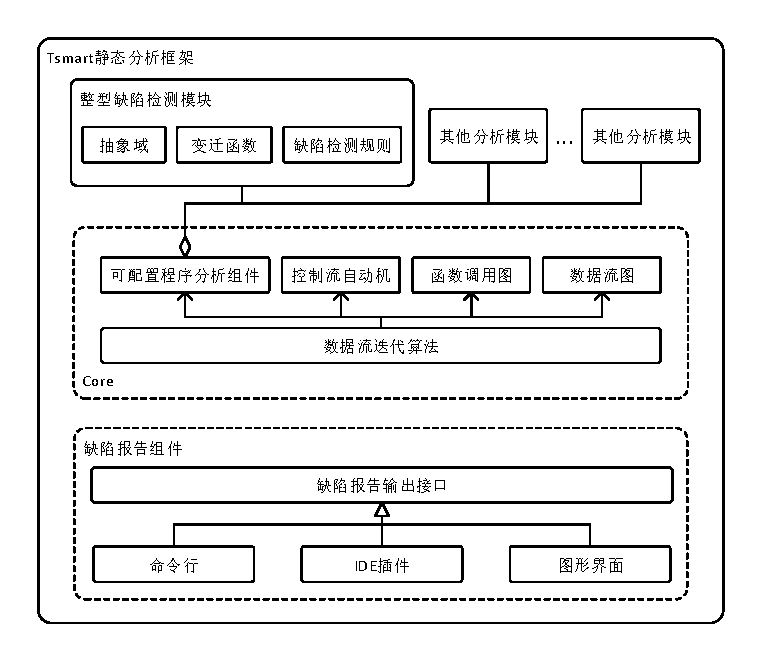
\includegraphics{ZhengXingFenXi_JiaGouTu.pdf}
	\caption{整型缺陷分析工具架构图}
	\label{fig:整型分析架构图}
\end{figure}

本模块的实现基于Tsmart静态分析框架,分析框架的输入是C语言源代码,工具的前端程序将C语言代码转化为具有静态单赋值特性的LLVM-IR语言,并在得到的LLVM-IR上构造与之等价的控制流自动机(CFA)。

本模块借助Tsmart提供的接口来获取生成的CFA并以此为基础进行抽象域与检测算法的实现。我们按照前几个小节对理论域RangeInteger、Range、MultiRange、SignRange以及RangeState的介绍,在框架上依次实现其定义及计算规则,同时实现RangeState的状态变迁规则。理论域在工具上的实现结构同图\ref{fig:Domains}。

为了实现整型缺陷检测,我们按照规则\ref{align:overflow}、\ref{align:underflow}和\ref{align:dividebyzero}实现检测规则,并通过调用分析框架提供的缺陷报告输出接口实现整型缺陷的输出。

\subsection{实验设计}

为了客观评价本章提出的整型缺陷检测方法,我们选用Juliet Test Suite测试集作为本工具的检测样本。Juliet测试集由美国国家标准技术研究所 (NIST) 整理出的C语言上包含各类标准错误的样例代码集合。针对每一类定义在CWE上的程序缺陷,Juliet有对应的文件夹包含了在不同情境下出现这类错误的情况。

本次实验选用Juliet测试集中的CWE190\_Integer\_Overflow、CWE191\_Integer\_Underflow和CWE369\_Divide\_by\_Zero三类缺陷样例,其中,CWE190包含7个从测试集s01到s07共3420个测试样例;CWE191包含5个从测试集s01到s05共2622个测试样例;CWE369包含测试集s01、s02共684个测试样例。Juliet测试集为同种缺陷设计了多种多样的发生环境,包括:不同字节长度、不同符号性(有符号数和无符号数)、结构体、枚举、函数调用、循环等。同时,对应的情景也不尽相同,如套接字应用场景、标准输入输出场景、随机数生成等。

如图\ref{fig:example_bad}和图\ref{fig:example_good}所示代码来自Juliet测试集中的一个简单的测试样例,我们以此介绍如何使用Juliet测试集对工具进行评估。该样例用于测试缺陷检测工具对整型上溢出缺陷的检测能力。具体地,它试图对char类型的变量data进行加1操作。图\ref{fig:example_good}包含了正确的两个函数实现:函数goodG2B中data的取值来自常量赋值,该赋值保证变量data的加1操作不会上溢出;函数goodB2G中data的取值来自标准输入,在加法操作前检验了data的取值,确认加1操作不会产生溢出。在图\ref{fig:example_bad}所示代码中,data的取值来自标准输入,在加法运算之前并未进行溢出检验,存在整型溢出缺陷。

Juliet测试集中,所有正确实现的函数均以“xxx\_xxx\_good”命名,所有包含缺陷的函数均以“xxx\_xxx\_bad”命名。借此,我们可以方便的对工具的检测结果进行评估:若函数实现中存在缺陷,但未在缺陷报告中出现,或缺陷定位不准确的,记为漏报;若函数实现准确,但在缺陷报告中出现,则记为误报。本次实验依次将上述测试集的测试样例作为输入,记录工具对各个样例的测试结果并统计误报率、漏报率以及对应的测试时间,以此评估工具的准确性与可用性。实验结果将于\ref{sec:区间算数实验结果}小节中给出。

\begin{figure}[H]
	\centering
	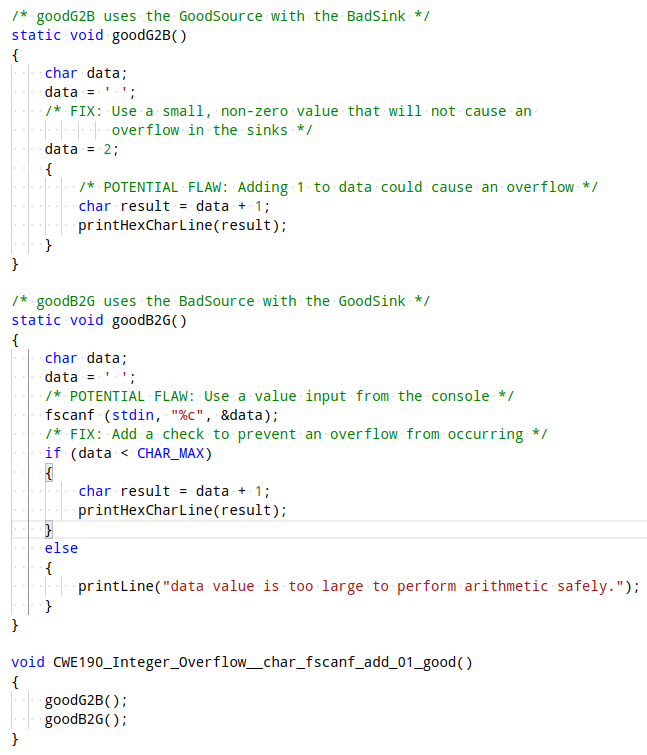
\includegraphics{example_good.png}
	\caption{Juliet测试集测试样例举例(正例)}
	\label{fig:example_good}
\end{figure}

\begin{figure}[H]
	\centering
	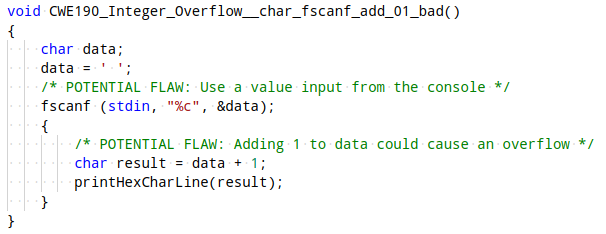
\includegraphics{example_bad.png}
	\caption{Juliet测试集测试样例举例(负例)}
	\label{fig:example_bad}
\end{figure}



本次实验的运行环境列举如下:
\begin{itemize}
	\item 操作系统:Ubuntu 16.04 LTS 64位版本
	\item 处理器:Intel(R) Core(TM) i7-6500U@2.50GHz 4核心CPU
	\item 内存大小:16GB
\end{itemize}

\subsection{实验结果}
\label{sec:区间算数实验结果}

本章介绍的整型缺陷检测工具在Juliet测试集上的测试结果如表\ref{tab:190Result}(CWE190测试结果)、表\ref{tab:191Result}(CWE191测试结果)和表\ref{tab:369Result}(CWE369测试结果)所示:

\begin{longtable}{ccccccc}
	\caption[CWE190测试结果]{CWE190测试结果}
	\label{tab:190Result}  \\ % add \\ command to tell LaTeX to start a new line	
	
	% Appear table header at the first page as well
	\toprule[1.5pt]	
	{\heiti 测试集} & {\heiti 总数} & {\heiti 误报} & {\heiti 漏报} & {\heiti 误报率} & {\heiti 漏报率} & {\heiti 运行时间} \\
	\midrule[1pt]
	\endfirsthead
	
	% Appear the table header at the top of every page
	\multicolumn{7}{c}{续表~\thetable\hskip1em CWE190测试结果}\\
	\toprule[1.5pt]	
	{\heiti 测试集} & {\heiti 总数} & {\heiti 误报} & {\heiti 漏报} & {\heiti 误报率} & {\heiti 漏报率} & {\heiti 运行时间} \\
	\midrule[1pt]
	\endhead 
	
	% Appear \hline at the bottom of every page
	\hline
	\multicolumn{7}{r}{续下页}
	\endfoot 
	\endlastfoot
	
	% data begins here	
	S01	& 418&	11&	0	&0.026315789&	0 & 7m 49s	\\
	S02	&418&	11&	0	&0.026315789&	0 & 7m 37s	\\
	S03	&418&	11&	0	&0.026315789&	0 & 7m 54s	\\
	S04	&418&	11&	0	&0.026315789&	0 & 7m 47s 	\\
	S05	&380&	10&	0	&0.026315789&	0 &	8m 31s	\\
	S06	&684&	18&	0	&0.026315789&	0 &	15m 42s\\
	S07	&684&	18&	0	&0.026315789&	0 &	16m 2s\\
	% more data here
	\bottomrule[1.5pt]
\end{longtable}

\begin{longtable}{ccccccc}
	\caption[CWE191测试结果]{CWE191测试结果}
	\label{tab:191Result}  \\ % add \\ command to tell LaTeX to start a new line	
	
	% Appear table header at the first page as well
	\toprule[1.5pt]	
	{\heiti 测试集} & {\heiti 总数} & {\heiti 误报} & {\heiti 漏报} & {\heiti 误报率} & {\heiti 漏报率}& {\heiti 运行时间}  \\
	\midrule[1pt]
	\endfirsthead
	
	% Appear the table header at the top of every page
	\multicolumn{7}{c}{续表~\thetable\hskip1em CWE191测试结果}\\
	\toprule[1.5pt]	
	{\heiti 测试集} & {\heiti 总数} & {\heiti 误报} & {\heiti 漏报} & {\heiti 误报率} & {\heiti 漏报率}& {\heiti 运行时间}  \\
	\midrule[1pt]
	\endhead 
	
	% Appear \hline at the bottom of every page
	\hline
	\multicolumn{7}{r}{续下页}
	\endfoot 
	\endlastfoot
	
	% data begins here	
	S01	&418	&11	&0	&0.026315789	&0	& 8m 23s	\\
	S02	&418	&11	&0	&0.026315789	&0	& 8m 8s	\\
	S03	&418	&11	&0	&0.026315789	&0	& 8m 50s	\\
	S04	&684	&18	&0	&0.026315789	&0	& 13m 57s	\\
	S05	&684	&18	&0	&0.026315789	&0	& 13m 9s	\\
	% more data here
	\bottomrule[1.5pt]
\end{longtable}

\begin{longtable}{ccccccc}
	\caption[CWE369测试结果]{CWE369测试结果}
	\label{tab:369Result}  \\ % add \\ command to tell LaTeX to start a new line	
	
	% Appear table header at the first page as well
	\toprule[1.5pt]	
	{\heiti 测试集} & {\heiti 总数} & {\heiti 误报} & {\heiti 漏报} & {\heiti 误报率} & {\heiti 漏报率} & {\heiti 运行时间}  \\
	\midrule[1pt]
	\endfirsthead
	
	% Appear the table header at the top of every page
	\multicolumn{7}{c}{续表~\thetable\hskip1em CWE369测试结果}\\
	\toprule[1.5pt]	
	{\heiti 测试集} & {\heiti 总数} & {\heiti 误报} & {\heiti 漏报} & {\heiti 误报率} & {\heiti 漏报率} & {\heiti 运行时间}  \\
	\midrule[1pt]
	\endhead 
	
	% Appear \hline at the bottom of every page
	\hline
	\multicolumn{7}{r}{续下页}
	\endfoot 
	\endlastfoot
	
	% data begins here	
	S01	&418	&11	&0	&0.026315789	&0 & 6m 58s	\\
	S02	&266	&7	&0	&0.026315789	&0	& 4m 35s\\
	% more data here
	\bottomrule[1.5pt]
\end{longtable}

通过表中数据可以看出,本章提出的基于区间运算的整型缺陷分析工具在Juliet-190、191、369上的测试结果良好:误报率小于3\%,漏报率为0\%。其中,造成误报的原因是Tsmart静态分析框架在处理for循环时使用了循环摘要策略,导致整型变量在抽象域上的计算结果有一定的精度丢失。

在分析框架处理循环时,常常需要对循环做摘要处理。这在处理具体问题时是非常有好处的:它避免因循环展开而造成的分析时间不确定的问题,甚至规避了无限次循环展开的情形。为了得到循环摘要,常用的做法是使用循环不变式来计算各个整型变量在循环中的行为,进而计算得到结果。工具的后续研究方向是优化循环不变式的求解,从而获得更高的分析精度。

从分析效率上看,工具在各个测试集上的分析时间均小于10分钟,平均每个测试样例的分析时间小于2秒。具有实际应用价值。

\section{基于值流图的整型变量关系分析方法的实现与评估}
\label{sec:值流图评估与结果}

\subsection{工具实现}

虑到根据源代码生成精确值流图的过程十分复杂,基于值流图的整型变量关系分析的实现基于Tsmart静态分析框架,它的优点是使用静态分析的方法,高效的生成控制流自动机和精确值流图。同时该分析框架具有可配置性,能够较容易的获取到所需程序上下文信息,因此我们采用此分析框架,工具的开发语言为Java,工具的框架图如图\ref{fig:架构图}所示。

\begin{figure}[H]
	\centering
	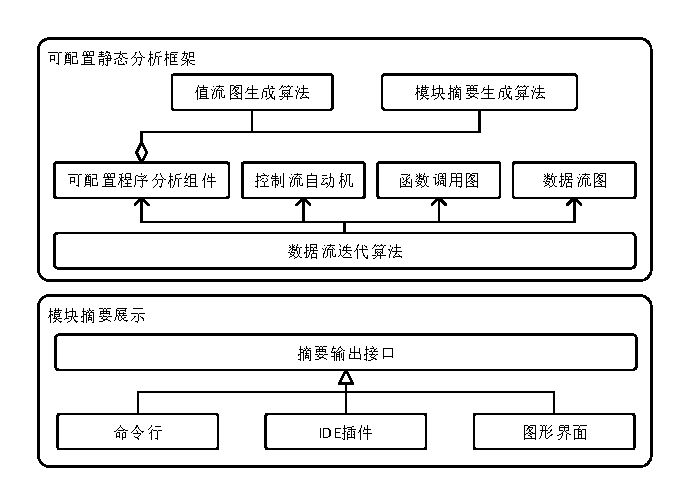
\includegraphics[width=6in]{JiaGouTu.pdf}
	\caption{工具架构图}
	\label{fig:架构图}
\end{figure}

借助Tsmart静态分析框架,我们可以快速构建第\ref{sec:值流图}章节所介绍的整型变量关系的抽象域并实现其变迁关系。同时,利用Tsmart框架提供的相应接口,我们可以生成所需的值流图,并以此为基础实现整型变量关系分析算法。

在后两个小节,我们将从客观、主观两个方面评估算法(工具)在程序理解与需求确认方面的效用。客观评价重点关注算法的完整性与准确性。具体而言,我们考察算法自动生成的摘要质量;主观评价则重点关注工具在具体的生产环境中的可用性与实用性。我们将分别从客观评价和主观评价两个方面对工具进行实验。

\subsection{客观评价}

客观评价方法主要包含以下几个步骤:(1)分别选取数学计算、计算机应用、工业领域和嵌入式领域中8个具有代表性的代码片段作为实验对象(详见表\ref{tab:selectedCodes});(2)采用本文工具分别生成相应的函数摘要;(3)判定工具自动生成的摘要与实际需求的差距。
\begin{longtable}{ccc}
	\caption{选取的各类代码}
	\label{tab:selectedCodes}  \\ % add \\ command to tell LaTeX to start a new line	
	
	% Appear table header at the first page as well
	\toprule[1.5pt]	
	{\heiti 类别} & {\heiti 选取代码}  & {\heiti 文件名称}  \\
	\midrule[1pt]
	\endfirsthead
	
	% Appear the table header at the top of every page
	\multicolumn{3}{c}{续表~\thetable\hskip1em 选取的各类代码}\\
	\toprule[1.5pt]	
	{\heiti 类别} & {\heiti 选取代码}  & {\heiti 文件名称}  \\
	\midrule[1pt]
	\endhead 
	
	% Appear \hline at the bottom of every page
	\hline
	\multicolumn{3}{r}{续下页}
	\endfoot 
	\endlastfoot
	
	% data begins here	
	\multirow{2}{*}{数学计算} & 三角形判定 & triangle.c \\ 
	& 绝对值计算 & abs.c \\ 
	\multirow{2}{*}{计算机应用} & (加权平均)滤波算法 & filter.c \\ 
	& 校验和算法 & checksum.c \\ 
	\multirow{2}{*}{工业领域} & 车辆控制系统某算法 & CDL\_ARC429.c \\ 
	& 航天发动机控制系统某算法 & ISP\_TOOL.c \\
	\multirow{2}{*}{嵌入式领域} & 含goto语句的程序片段 & msp430-decode.c \\
	& 带函数指针的程序片段 & xen-ops.c \\ 
	% more data here
	\bottomrule[1.5pt]
\end{longtable}
%\begin{table}[htb]
%	\centering
%	\caption{选取的各类代码}
%	\label{tab:selectedCodesxx}
%	\begin{tabular}{|c|c|c|}
%		\hline
%		类别 & 选取代码 & 文件名称 \\ \hline
%		\multirow{2}{*}{数学计算} & 三角形判定 & triangle.c \\ \cline{2-3} 
%		& 绝对值计算 & abs.c \\ \hline
%		\multirow{2}{*}{计算机应用} & (加权平均)滤波算法 & filter.c \\ \cline{2-3} 
%		& 校验和算法 & checksum.c \\ \hline
%		\multirow{2}{*}{工业领域} & 车辆控制系统某算法 & CDL\_ARC429.c \\ \cline{2-3} 
%		& 航天发动机控制系统某算法 & ISP\_TOOL.c \\ \hline
%		\multirow{2}{*}{嵌入式领域} & 含goto语句的程序片段 & msp430-decode.c \\ \cline{2-3} 
%		& 带函数指针的程序片段 & xen-ops.c \\ \hline
%	\end{tabular}
%\end{table}

由于摘要结果和程序的条件分支有关,因此本文分别对比两者在每个条件分支下的生成结果。同时,记录工具的时间和空间开销,包括摘要生成时间、占用内存大小以及生成的VFG大小,如表\ref{tab:summaryComparision}所示。

\begin{table}[htb]
	\centering
	\caption{自动生成摘要和人工生成摘要的对比}
	\label{tab:summaryComparision}
	\begin{tabular}{cccccccc}
		\toprule[1.5pt]	
		\multicolumn{2}{c}{\heiti 程序代码} & {\heiti 实际需求} & \multicolumn{4}{c}{\heiti 自动摘要} & \multirow{2}{*}{\begin{tabular}[c]{@{}c@{}}{\heiti 正确}\\ {\heiti 率}\end{tabular}} \\ \cline{1-7}
		类型 & 代码行 & 分支数 & 分支数 & 耗时/s & 内存/MB & VFG大小/KB &  \\ \midrule[1pt]
		三角形判定 & 24 & 4 & 4 & 3 & 134 & 9 & 1.0 \\ 
		绝对值 & 11 & 2 & 2 & 2 & 122 & 2 & 1.0 \\ 
		滤波算法 & 19 & 1 & 1 & 2 & 128 & 4 & 1.0 \\ 
		校验和算法 & 22 & 1 & 1 & 2 & 145 & 12 & 1.0 \\ 
		车辆控制系统 & 124 & 12 & 12 & 5 & 167 & 53 & 1.0 \\ 
		航发控制系统 & 178 & 15 & 15 & 6 & 171 & 61 & 1.0 \\ 
		Goto语句 & 57 & 8 & 8 & 4 & 137 & 34 & 1.0 \\ 
		函数指针 & 36 & 3 & 3 & 3 & 132 & 6 & 1.0 \\
		\bottomrule[1.5pt]
	\end{tabular}
\end{table}

经实验验证,本工具能够完整地生成不同类型代码的摘要,且生成摘要的条件分支数与需求一致。运行工具所消耗的资源相对较少,内存占用小于200MB,生成的VFG均小于1MB。工具可以较快的生成函数摘要,生成百行级别代码所需时间不超过1分钟。

\subsection{主观评价}

为保证主观评价的公平性与准确性,现从学校选取共30名条件相当的同学参与实验,他们均符合以下条件:(1)拥有超过3年的C语言编程经验,且均使用C语言通过了学校的编程水平测验;(2)对表\ref{tab:selectedCodes}代码所在的背景了解程度相当。

实验方法包含以下几个步骤:(1)将30名同学分为源码组和摘要组进行对照实验,分别为其提供表5所示的8份源代码(或含摘要的源代码);(2)令每名同学阅读代码,并令其说出代码功能,记录用时T1;(3)令每名同学分析函数在不同输入的情况下的输出,记录用时T2;(4)分别统计并对比两组同学在不同代码上回答问题所用时间T1和T2的平均值;(5)在源码组同学完成后,为其提供摘要。同时分别询问两组同学对摘要的看法。 

如表\ref{tab:ComprehensionComparision}所示为两组同学在各个代码上回答实验步骤2和3中提出问题的平均用时T1和T2。通过对比可知,在代码行数较小(10行以内)且逻辑并不复杂的情况下,使用摘要对程序理解无明显帮助。但当面对几十甚至上百行代码时,使用摘要可明显减少用户理解代码所用时间。在含goto语句的实验样本上,可节省60.5\%的程序理解时间。

通过实验可知,本工具可显著提高用户对代码的理解效率,能够帮助用户快速抽取程序语义并进行需求确认。同时,随着代码分支复杂度的提升,使用工具进行程序理解与需求确认的优势将越来越大。

\begin{longtable}{ccccc}
	\caption{各组对每类代码理解并作答所用时间}
	\label{tab:ComprehensionComparision}  \\ % add \\ command to tell LaTeX to start a new line	
	
	% Appear table header at the first page as well
	\toprule[1.5pt]	
	{\heiti 程序代码} & {\heiti 源码组T1/s}  & {\heiti 源码组T2/s}  & {\heiti 摘要组T1/s}  & {\heiti 摘要组T2/s}    \\
	\midrule[1pt]
	\endfirsthead
	
	% Appear the table header at the top of every page
	\multicolumn{5}{c}{续表~\thetable\hskip1em 选取的各类代码}\\
	\toprule[1.5pt]	
	{\heiti 程序代码} & {\heiti 源码组T1/s}  & {\heiti 源码组T2/s} & {\heiti 摘要组T1/s}   & {\heiti 摘要组T2/s}    \\
	\midrule[1pt]
	\endhead 
	
	% Appear \hline at the bottom of every page
	\hline
	\multicolumn{5}{r}{续下页}
	\endfoot 
	\endlastfoot
	
	% data begins here	
	三角形判定 & 45 & 32 & 37 & 14 \\ 
	绝对值 & 5 & 13 & 11 & 14 \\ 
	滤波算法 & 61 & 15 & 27 & 15 \\ 
	校验和算法 & 97 & 43 & 54 & 38 \\ 
	车辆控制系统 & 294 & 86 & 103 & 74 \\ 
	航发控制系统 & 318 & 92 & 114 & 91 \\ 
	Goto语句 & 195 & 48 & 64 & 31 \\ 
	函数指针 & 82 & 33 & 40 & 29 \\ 
	% more data here
	\bottomrule[1.5pt]
\end{longtable}
%\begin{table}[htb]
%	\centering
%	\caption{各组对每类代码理解并作答所用时间}
%	\label{tab:ComprehensionComparisionxx}
%	\begin{tabular}{|c|c|c|c|c|}
%		\hline
%		程序代码 & 源码组T1/s & 源码组T2/s & 摘要组T1/s & 摘要组T2/s \\ \hline
%		三角形判定 & 45 & 32 & 37 & 14 \\ \hline
%		绝对值 & 5 & 13 & 11 & 14 \\ \hline
%		滤波算法 & 61 & 15 & 27 & 15 \\ \hline
%		校验和算法 & 97 & 43 & 54 & 38 \\ \hline
%		车辆控制系统 & 294 & 86 & 103 & 74 \\ \hline
%		航发控制系统 & 318 & 92 & 114 & 91 \\ \hline
%		Goto语句 & 195 & 48 & 64 & 31 \\ \hline
%		函数指针 & 82 & 33 & 40 & 29 \\ \hline
%	\end{tabular}
%\end{table}

在实验步骤5中,我们设计了数道问题,交予参与实验的同学回答并统计,最终得到的结果如表\ref{tab:questionaire}。实验参与者对自动生成摘要工具总体持肯定态度,认为生成的摘要对理解代码有帮助。对于摘要是否可以帮助分析变更影响范围与帮助软件维护方面,一部分同学持观望和怀疑态度,认为本工具生成的摘要为函数级别的摘要,而变更影响范围分析与软件维护可能涉及全局代码,需要结合函数调用等信息进一步分析。

\begin{longtable}{cccc}
	\caption{问卷设计与答复情况}
	\label{tab:questionaire}  \\ % add \\ command to tell LaTeX to start a new line	
	
	% Appear table header at the first page as well
	\toprule[1.5pt]	
	{\heiti 问题设计} & {\heiti 赞同人数}  & {\heiti 否定人数}  & {\heiti 其他想法}  \\
	\midrule[1pt]
	\endfirsthead
	
	% Appear the table header at the top of every page
	\multicolumn{4}{c}{续表~\thetable\hskip1em 问卷设计与答复情况}\\
	\toprule[1.5pt]	
	{\heiti 问题设计} & {\heiti 赞同人数}  & {\heiti 否定人数}  & {\heiti 其他想法}  \\
	\midrule[1pt]
	\endhead 
	
	% Appear \hline at the bottom of every page
	\hline
	\multicolumn{4}{r}{续下页}
	\endfoot 
	\endlastfoot
	
	% data begins here	
	摘要是否有助于你理解代码? & 28 & 2 & 0 \\
	你认为摘要是否对影响范围分析有帮助? & 25 & 4 & 1 \\ 
	你认为摘要是否对软件维护有帮助? & 22 & 7 & 1 \\ 
	% more data here
	\bottomrule[1.5pt]
\end{longtable}
%\begin{table}[htb]
%	\centering
%	\caption{问卷设计与答复情况}
%	\label{tab:questionairexx}
%	\begin{tabular}{|c|c|c|c|}
%		\hline
%		问题设计 & 赞同人数 & 否定人数 & 其他想法 \\ \hline
%		摘要是否有助于你理解代码? & 28 & 2 & 0 \\ \hline
%		你认为摘要是否对影响范围分析有帮助? & 25 & 4 & 1 \\ \hline
%		你认为摘要是否对软件维护有帮助? & 22 & 7 & 1 \\ \hline
%	\end{tabular}
%\end{table}

\section{本章小结}

本章介绍了基于线性区间的整型缺陷检测方法与基于精确值流图的整型变量关系分析方法的具体实现方法与相关实验设计。同时,我们对得到的实验结果进行了评价并分析造成误报与精度损失的原因。

在基于线性区间的整型缺陷检测的实验中,测试用例的误报主要原自基于for循环的检测,而现有框架对循环的处理基于循环摘要。由于循环摘要的精度受制于循环不变式技术,因此为了进一步提升整型缺陷分析在循环中的精度,本文后续的工作重点将集中在循环不变式上。

另一方面,基于精确值流图的整型变量关系分析方法依赖于精确值流图的准确生成,当前可用工具相对较少,且在面对大型程序时消耗的时间空间较多。这会对本工具的结果造成一定影响。一个可能的解决方案是在原有的值流图算法上进行优化,针对于循环与数组,优化其结果。此外,为了保证算法的收敛性与时间开销,算法在处理循环时,引入了符号值$ \mu $,算法的结果是带$ \mu $的符号表达式,这将在处理循环时带来一定的精度丢失。后续可以使用循环不变式等技术进一步提高分析精度。同时,为了增强工具对全局影响范围的分析,后续将会结合函数调用等信息,提升工具的适用性。





































